\documentclass{template/openetcs_article}
% Use the option "nocc" if the document is not licensed under Creative Commons
%\documentclass[nocc]{template/openetcs_article}
\usepackage{lipsum,url}
\graphicspath{{./template/}{.}{./images/}}
\begin{document}
\frontmatter
\project{openETCS}

%Please do not change anything above this line
%============================
% The document metadata is defined below

%assign a report number here
\reportnum{OETCS/WP3/SysML Modeling with Papyrus}

%define your workpackage here
\wp{Work-Package 3: "Modeling''}

%set a title here
\title{Guidelines for SysML modeling with Papyrus \\ Model Documentation}

%set a subtitle here
\subtitle{This document aims at describing the Papyrus tool usage in the frame of the OBU EVC software modelisation.}

%set the date of the report here
\date{July 2013\\Revised August 2013}

%define a list of authors and their affiliation here

\author{Alexandre Ginisty}

\affiliation{All4tec\\
  Immeuble Odyssée Bâtiment E  \\
2-12, Rue du Chemin des femmes \\ 
91 300 MASSY, France}


% define the coverart
\coverart[width=350pt]{chart}

%define the type of report
\reporttype{Description of work}


\begin{abstract}
This document provides the methodology and the use of the modeling tool Papyrus, in order to model the OBU EVC Software with UML/ SysML language.
It is willing to support the good practices, knowledges, and overall modeling methodology, and spread them out to the project. In accordance with the open source philosophy, this methodology is willing to be transparently shared with all modelers involved in the project, and to be an alive support for modeling. Every modeler is invited to provide additional informations regarding the methods or use of Papyrus, in order improve this document and to make out of it a real user manual for OBU EVC modeling with Papyrus.

\end{abstract}

%=============================
%Do not change the next three lines
\maketitle
\tableofcontents
\listoffiguresandtables
\newpage
%=============================

% The actual document starts below this line
%=============================




\section{Short Introduction to Formalism and Tool}
This document describes the modeling of the On-Sight Procedure. The mode has been made from the specification description of the SRS SUBSET-026-3.5 baseline 3 as recommended by D2.5 Methods and tools benchmarking methodology.
The formalism used is SysML . More particularly we had used block diagram, state charts and activity diagrams. SysML is a graphical language that extends UML for a customize version suitable for system engineering. It may help modeling system within a board range of system variety that may include hardware, software, data, personnel and facilities. It supports the specification, analysis design, verification and validation of complex system.
Papyrus is an open source tool that has been used to implement the model. Papyrus is aiming at providing an integrated and user-consumable environment for editing any kind of EMF model and particularly supporting UML and related modeling languages such as SysML and MARTE.
The main feature of Papyrus regarding this latter point is a set of very powerful customization mechanisms which can be leveraged to create user-defined Papyrus perspectives and give it the same look and feel as a native DSL editor.
This model is currently not executable or testable but its transformation is scheduled.

\begin{figure}[h]
  \centering
  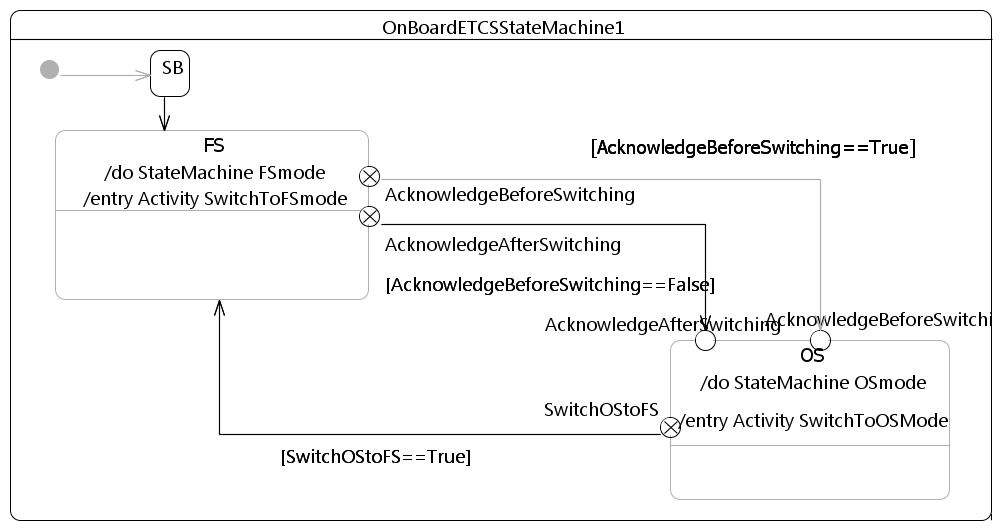
\includegraphics[width=14cm]{fig1_example_on_diagram_used.png}
  \caption{Example of diagram used}
  \label{fig: Example of diagram used}
\end{figure}

\section{Prerequisites}
This section shortly describes the basic prerequisites to use Papyrus projects on github.
\subsection{Papyrus platform}
This model has been made on Papyrus under Eclipse platform version Juno available here: http://www.eclipse.org/downloads/packages/eclipse-modeling-tools/junosr1
To download Papyrus, launch Eclipse, go to “Help -> Install Modeling Component” and select Papyrus.

\subsection{Importing an existing Papyrus project :}
Papyrus projects are composed of 4 files, “.project”, “.uml”, “.notation” and “.di”. To import an existing Papyrus project, launch Papyrus, click on “File >> Import >> Existing project into Workspace”.
\newpage

\begin{figure}[h!]
  \centering
  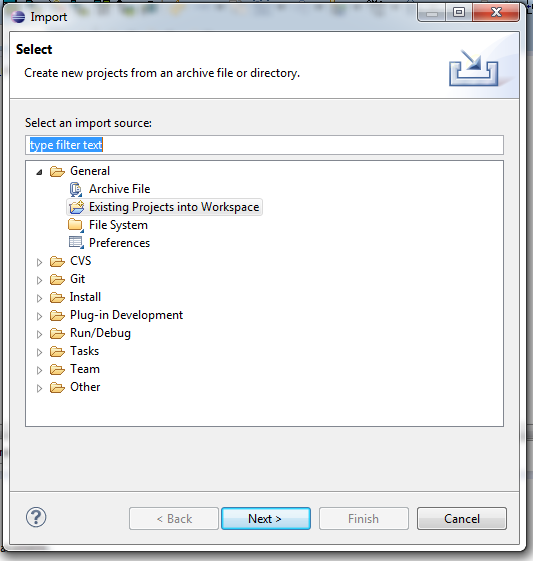
\includegraphics[width=10cm]{fig2_menu_import.png}
  \caption{Menu "Import"}
  \label{fig: Menu "Import"}
\end{figure}

Then Browse to the directory to select the project and click on Finish.

\begin{figure}[h!]
  \centering
  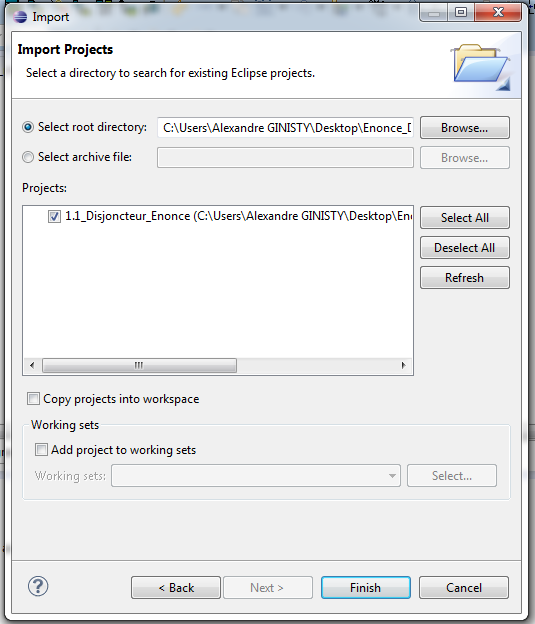
\includegraphics[width=10cm]{fig3_importing_existing_project.png}
  \caption{Importing existing project}
  \label{fig: Importing existing project}
\end{figure}

\section{Modeling Strategy }
A procedure like the On Sight procedure can be described in first approach in a SysML Sequence Diagram. It gives a better understanding, and allows to pinpoint which parts and which functions are involved in this procedure.
Then, based on Subset 026, we made block diagrams to model the whole system. Then we decided that, for a benchmark purpose, a simplified system will be better, and we modeled it.
The current model uses 3 main parts, the on-board unit, the rbc and the driver. We decided to focus on the on-board unit to model its behavior. We also decided to choose the initial mode and the ending mode of the procedure, and we don’t consider any level change during the procedure.

\begin{figure}[h]
  \centering
  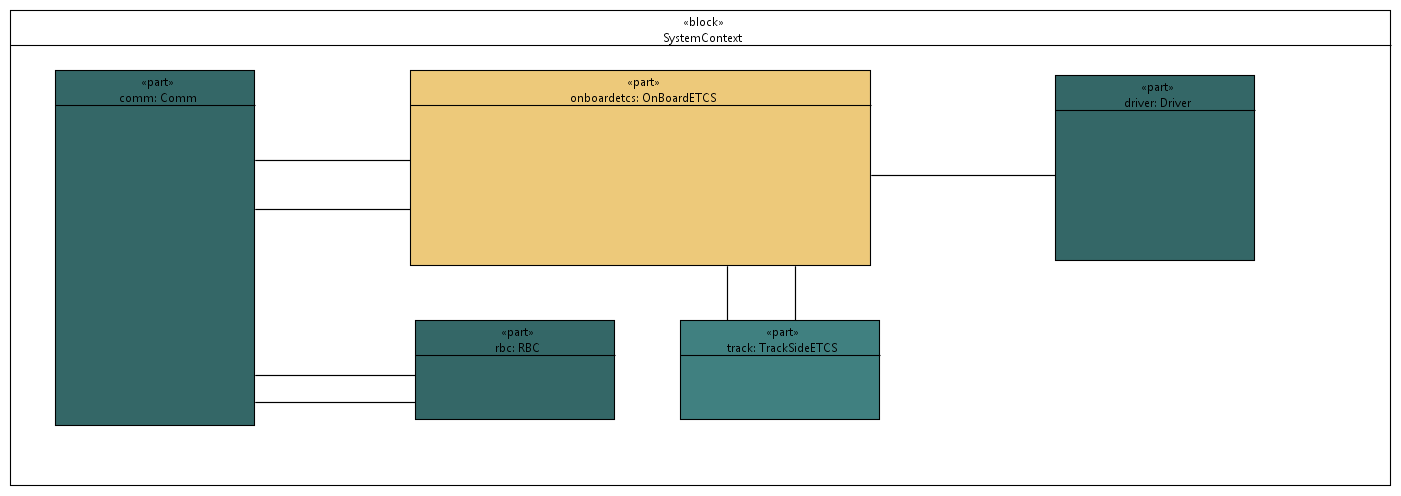
\includegraphics[width=14cm]{fig4_simplified_system_structure.png}
  \caption{Simplified system structure}
  \label{fig: Simplified system structure}
\end{figure}

\section{Model Overview}
There are 4 packages in the model but only two are used at the moment, the system model package and the System Requirements package.
The procedure is mainly described with statecharts. We started with sequence diagrams and activity diagrams, but found that the use of statecharts fill much our needs and can be more useful for further development (i.e using plugins for V\&V).
The procedure involves trackside means (RBC, Euroloop, etc.), the On Board unit (OBU) and the driver. On Sight mode request may come from trackside means, considering we can only be in Full Supervision mode when it comes (model restriction). In our model we only consider messages exchanged from OBU point of view.
\\
The overall behavior of On Board unit is modeled as below:
\begin{figure}[h]
  \centering
  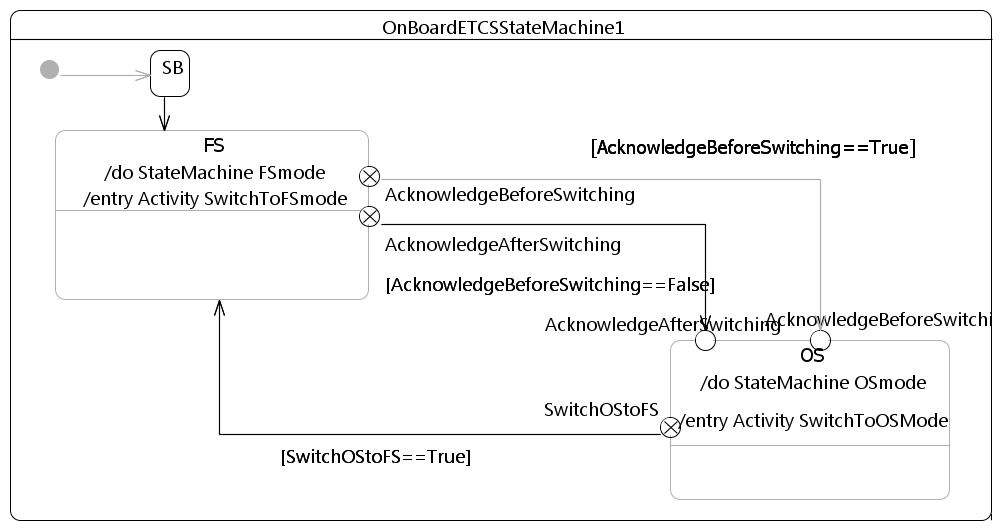
\includegraphics[width=14cm]{fig5_OBU_Behavior_mode_switching.png}
  \caption{OBU behavior for mode switching}
  \label{fig: OBU behavior for mode switching}
\end{figure}

Starting from SB mode for consistency, the OBU switch to FS mode. 

\begin{figure}[h]
  \centering
  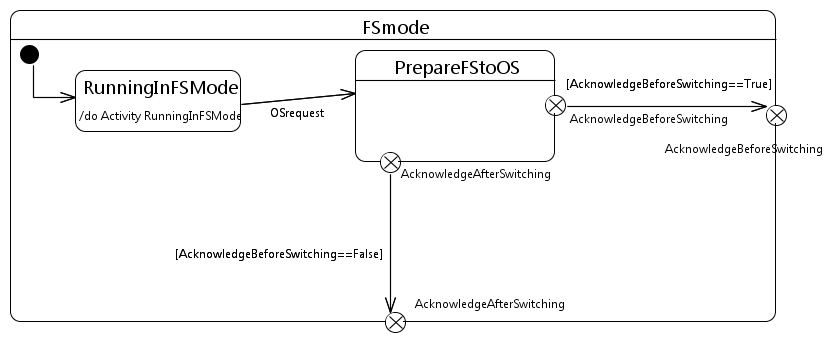
\includegraphics[width=10cm]{fig6_state_machine_fsmode.png}
  \caption{Sub-statemachine of FS mode}
  \label{fig: Sub-statemachine of FS mode}
\end{figure}

This Statechart models the first part of the procedure which concerne the OBU while it is in FS mode (OS request, Check conditions of displaying OS acknowledgement request, etc.)

\begin{figure}[h]
  \centering
  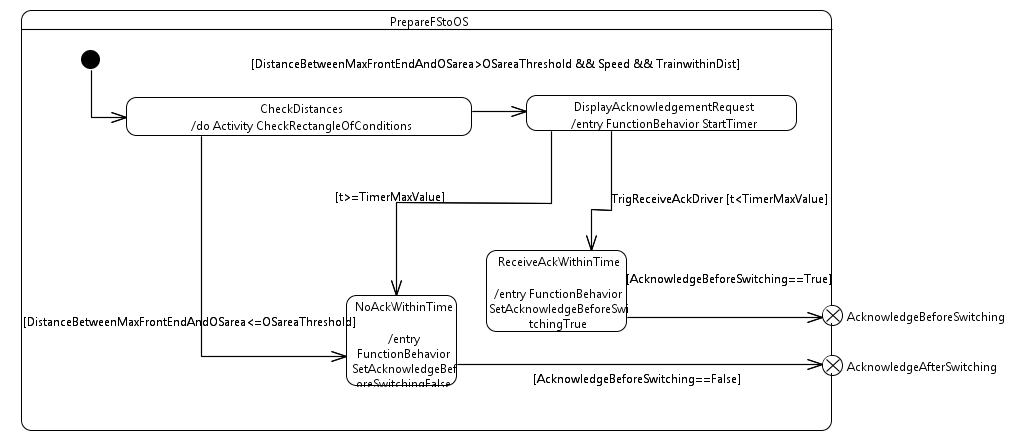
\includegraphics[width=14cm]{fig7_statechart_procedure.png}
  \caption{Statechart describing procedure from FS point of view}
  \label{fig: Statechart describing procedure from FS point of view}
\end{figure}

Activity diagrams are used to model low-level operations, such as checking the “rectangle of conditions”. The use of “Opaque Operation” has been made in order to model these operations without knowing exactly what they actually do.

\begin{figure}[h!]
  \centering
  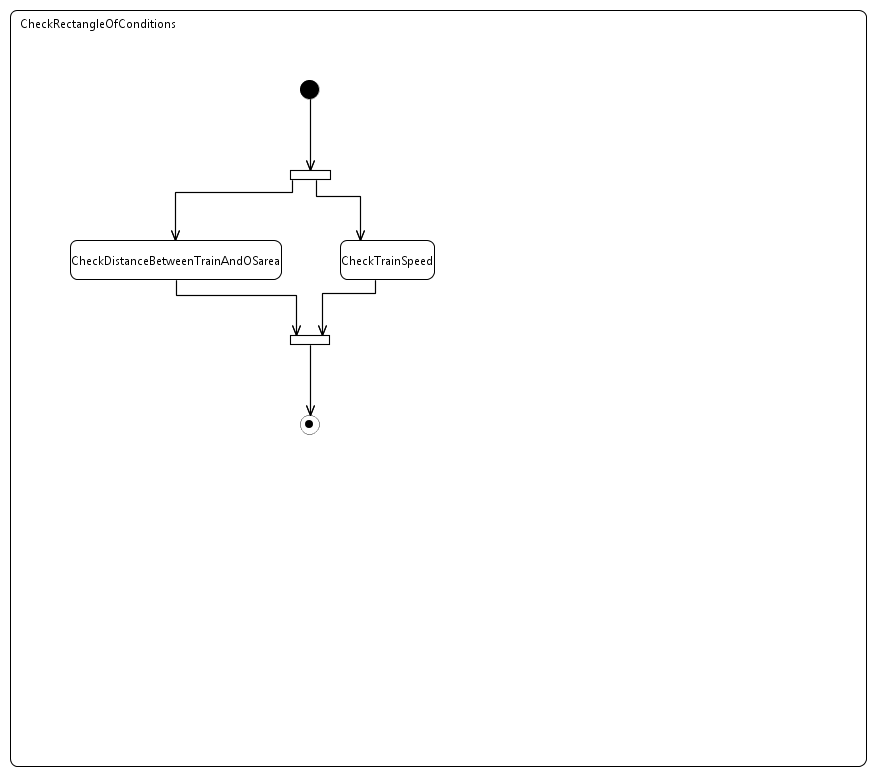
\includegraphics[width=14cm]{fig8_activity_diagram_check_conditions.png}
  \caption{Activity diagram for "Check rectangle of conditions}
  \label{fig: Activity diagram for "Check rectangle of conditions}
\end{figure}

\newpage

Notice that we decided to use the method of modeling that consider a distribution of the procedure between concerned modes, as it is described in Munich presentation (https://github.com/openETCS/model-evaluation/blob/master/Munich\_20130416/c\_Papyrus\_SysML\_V1.pdf)


\begin{figure}[h]
  \centering
  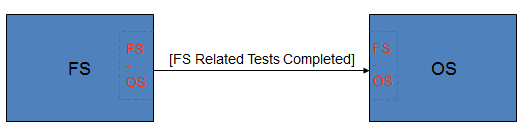
\includegraphics[width=10cm]{fig9_modeling_choice.png}
  \caption{Modeling choice using SysML}
  \label{fig: Modeling choice using SysML}
\end{figure}

Operations can be done during the entry or the exit of a state, or while the concerned state is active. Multiple choices are available for the location of the different operations and it needs experimentation to find which ones fit the most to reality.
Two conditional exits are possible, depending of the driver acknowledgement. They lead to two conditional entries in OS mode (OS Statechart).

\newpage

\begin{figure}[h]
  \centering
  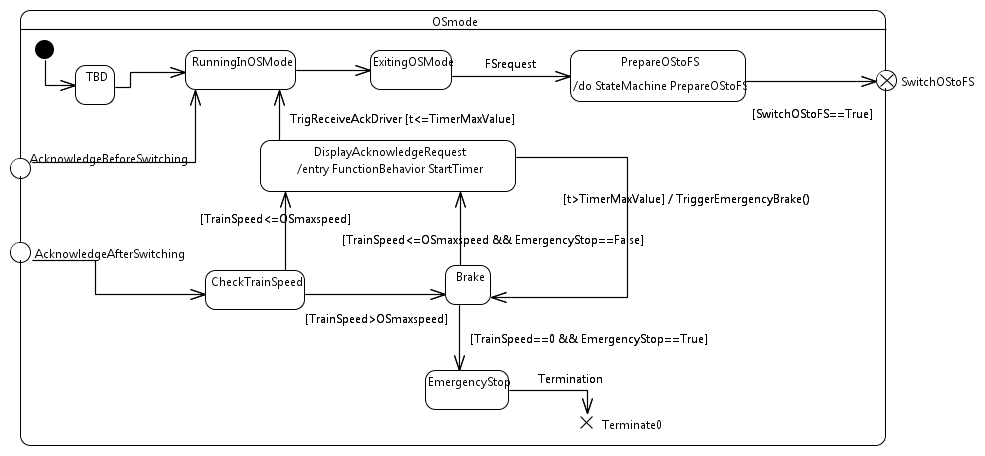
\includegraphics[width=14cm]{fig10_statechart_procedure_OS.png}
  \caption{Statechart describing procedure from OS point of view}
  \label{fig: Statechart describing procedure from OS point of view}
\end{figure}

In the same way, the procedure to switch from OS mode to FS mode is located in both modes (in fact, only in OS mode because of the procedure itself as it is described in Subset 026).

\begin{figure}[h]
  \centering
  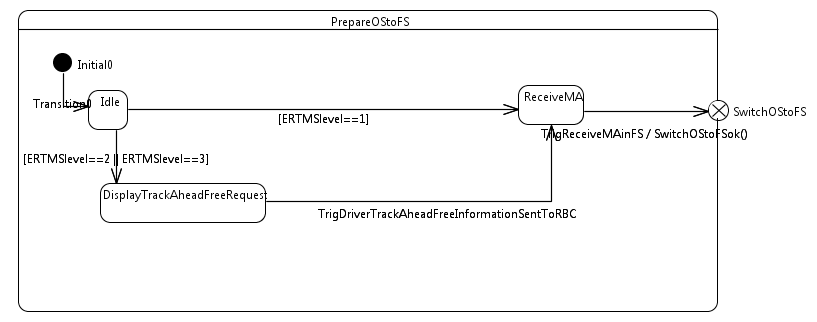
\includegraphics[width=14cm]{fig11_sub_statechart_OStoFS.png}
  \caption{Sub-statemachine describing OS to FS procedure}
  \label{fig: Sub-statemachine describing OS to FS procedure}
\end{figure}
Diagrams and states can be easily linked to other parts of the subset 026 related to « procedures », such as receiving a new MA (which can also be described using statecharts and activity diagrams). This insure that further development and integration is possible (considering using only SysML for that level of models).

\section{Model Benefits and shortcomings}

We think that using SysML provides these benefits:
\begin{itemize}
\item Graphical language, easy to understand with few explanations, useful for demonstration,
\item Requirement and structure traceability,
\item Facilitate proving behavior consistency at high level.
\end{itemize}
Also, using SysML with Papyrus provides these benefits:
\begin{itemize}
\item Open Source tool,
\item Eclipse based, allowing many plugins to interface with,
\item Constant improvement.
\end{itemize}
However, both SysML and Papyrus have their shortcomings.
SysML is a semi-formal language that is aimed at modeled systems at a high level. It allows many means of modeling that can have strong consequences for performances or even system behavior. That choices have to be defined at the beginning of the model to insure consistency between all the parts and all the modelers in SysML.
Papyrus, as it is based on Eclipse platform, can have performance problems when modeling big systems. Moreover, the GUI is not very user friendly at the moment and it can be difficult to model efficiently without a good basic knowledge of the tool.

\nocite{*}


%===================================================
%Do NOT change anything below this line

\end{document}
